\documentclass[aspectratio=169,11pt,svgnames,handout]{beamer}

\usepackage[english]{babel}
\usepackage{graphicx}
\usepackage{enumitem}
\usepackage{amsmath}
\usepackage{mathtools}
\usepackage{float}
\usepackage{tikz}
\usetikzlibrary{patterns,arrows.meta,calc,3d,angles}
\usepackage{tkz-euclide}
\tikzset{point style/.style = {%
  draw = black,
  inner sep = 0pt,
  shape = circle,
  minimum size = 5pt,
  fill = black
 }
}
\usepackage{enumitem}

\usepackage{caption}
\usepackage{subcaption}

% Flowchart stuff

\usepackage{pgfopts}
\usepackage{xcolor}
\usepackage{tcolorbox}

\usetheme[
 titlestyle=style2,
 titleformat=smallcaps,
 sectionstyle=plain,
 slidestyle=cyber,
 headingcolor=theme,
 block=transparent
]{trigon}

\title{Number Sets}
\date{\today}
\author{Adam Klepáč}
\institute[GEVO]{Gymnázium Evolution Jižní Město}
\biglogo[width=.2\textwidth]{logo}
\smalllogo[width=.1\textwidth]{logo}
\titlegraphic{
\includegraphics[height=\paperheight]{title.jpg}}

\def\subsectionname{}

% enumerate global settings
\setlist[enumerate,1]{label=\arabic*.}
\setlist[enumerate,2]{label=\alph*)}

% custom colors %
\definecolor{Tiber}{HTML}{0A2841}
\definecolor{Charlotte}{HTML}{C0F6F9}
\definecolor{PictonBlue}{HTML}{53D0EC}
\definecolor{CuriousBlue}{HTML}{228FC6}
\colorlet{tPrim}{PictonBlue}
\colorlet{tTheme}{Charlotte}
\colorlet{tSec}{Tiber}
\colorlet{tAccent}{Tiber}

\newcommand{\clt}{\textcolor{Tiber}}
\newcommand{\clc}{\textcolor{Charlotte}}
\newcommand{\clp}{\textcolor{PictonBlue}}
\newcommand{\clu}{\textcolor{CuriousBlue}}

\newcommand{\N}{\mathbb{N}}

\tcbset{
 boxsep=7pt,
 fonttitle=\sc,
 colframe=tGreyBg,
 colframe=tPrim,
 boxrule=1pt
}

\begin{document}
\titleframe

\begin{frame}
 \frametitle{Contents}
 \tableofcontents
\end{frame}

\section{Natural Numbers}

\begin{frame}
 \frametitle{Natural Numbers -- Intuition}
 \alert{Natural numbers} are intuitively objects which represent a
 \alert{quantity}.\\
 \pause
 They're the following set:
 \[
  \N = \{0,1,2,3,\ldots\}.
 \]
 \pause
 A good way to think about them is to view them as `\emph{collections of
 blocks}'. You get the next natural number by adding another block on top of the
 previous collection.
 \begin{center}
  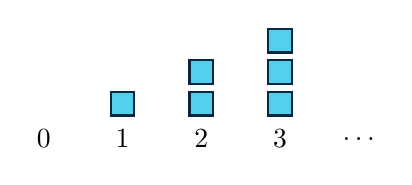
\begin{tikzpicture}
   \node at (0,-0.3) {$0$};

   \node at (1,-0.3) {$1$};
   \draw[draw=Tiber,thick,fill=PictonBlue] (0.85,0) rectangle ++(.3,.3);

   \node at (2,-0.3) {$2$};
   \draw[draw=Tiber,thick,fill=PictonBlue] (1.85,0) rectangle ++(.3,.3);
   \draw[draw=Tiber,thick,fill=PictonBlue] (1.85,0.4) rectangle ++(.3,.3);

   \node at (3,-0.3) {$3$};
   \draw[draw=Tiber,thick,fill=PictonBlue] (2.85,0) rectangle ++(.3,.3);
   \draw[draw=Tiber,thick,fill=PictonBlue] (2.85,0.4) rectangle ++(.3,.3);
   \draw[draw=Tiber,thick,fill=PictonBlue] (2.85,0.8) rectangle ++(.3,.3);

   \node at (4,-0.3) {$\ldots$};
  \end{tikzpicture}
 \end{center}
\end{frame}

\begin{frame}
 \frametitle{Natural Numbers -- Def\hspace*{0pt}inition}
 There are many ways to define natural numbers.\\
 \pause
 One of the popular ones is using a \alert{successor} function, denoted $s$.
 \pause
 If $n$ is a natural number, then $s(n)$ basically means `add another block on
 top of $n$'.\\
 \pause
 One would be of course tempted to write
 \[
  s(n) = n + 1
 \]
 but that \alert{doesn't make any sense}. We \alert{don't have addition yet}! In
 fact, you need the successor function to define addition in the first place.
\end{frame}

\begin{frame}
 \frametitle{Natural Numbers -- Def\hspace*{0pt}inition}
 The following \alert{five axioms} (often called \emph{Peano axioms}) constitute
 the definition of natural numbers:
 \pause
 \begin{enumerate}
  \item There exists the natural number $0$.
  \pause
  \item Every natural number has a successor which is also natural.
  \pause
  \item The number $0$ is not the successor of any natural number.
  \pause
  \item If $s(x) = s(y)$, then $x = y$.
  \pause
  \item (Induction Axiom) If a statement is true for $0$ and it being true for
   $n$ also implies that it is true for $n + 1$, then it is true for all natural
   numbers.
 \end{enumerate}
\end{frame}

\subsection{Unpacking The Axioms}

\begin{frame}
 \subsectionpage
\end{frame}

\begin{frame}
 \frametitle{Natural Numbers -- Axiom 1}
 \begin{center}
  \Large There exists the natural number $0$.\\
  \pause
  \vspace{\parskip}
  \normalsize\textcolor{gray!70}{Hopefully obvious.}
 \end{center}
\end{frame}

\begin{frame}
 \frametitle{Natural Numbers -- Axiom 2}
 \begin{center}
  \Large Every natural number has a successor which is also natural.\\
  \pause
  \vspace{\parskip}
  \normalsize\textcolor{gray!70}{Basically means that the natural numbers are an
  infinite set. You can add another block atop any collection of blocks.}
 \end{center}
\end{frame}

\begin{frame}
 \frametitle{Natural Numbers -- Axiom 3}
 \begin{center}
  \Large The number $0$ is not the successor of any natural number.\\
  \pause
  \vspace{\parskip}
  \normalsize\textcolor{gray!70}{Basically means that the natural numbers are
  infinite only `in one direction'. There is a \textbf{first} natural number.}
 \end{center}
\end{frame}

\begin{frame}
 \frametitle{Natural Numbers -- Axiom 4}
 \begin{center}
  \Large If $s(x) = s(y)$, then $x = y$.\\
  \pause
  \vspace{\parskip}
  \normalsize\textcolor{gray!70}{This means that the successor function is
  \textbf{injective} -- each natural number has a different successor.}
 \end{center}
\end{frame}

\begin{frame}
 \frametitle{Natural Numbers -- Axiom 5}
 \begin{center}
  \Large If a statement is true for $0$ and it being true for
   $n$ also implies that it is true for $n + 1$, then it is true for all natural
   numbers.\\
  \pause
  \vspace{\parskip}
  \normalsize\textcolor{gray!70}{This means that any feature of the natural
   numbers `propagates' via the successor function. Basically, if something is
   true for $0$ and we know that it is true for the next natural number if it is
   true for the previous one, then it is true for $1$ as well. Because it true
   for $1$, it is true for $2$ as well, etc.}
 \end{center}
\end{frame}

\subsection{Operations On Natural Numbers}

\begin{frame}
 \subsectionpage
\end{frame}

\begin{frame}
 \frametitle{What Is An Operation?}
 By \alert{operation}, we mean a function which takes \alert{one or multiple}
 natural numbers and produces \alert{one} natural number.\\
 \pause
 For example, $+$ and $ \cdot $ are operations because they take \alert{two}
 natural numbers and produce \alert{one}.\\
 \pause
 We don't often see them as functions because we don't write them as such. We
 write $a + b$ instead of $+(a,b)$ and $a \cdot b$ instead of $ \cdot (a,b)$.\\
 \pause
 In this sense, subtraction and division \alert{are not operations}! They take
 two natural numbers but they \alert{do not produce a natural number}.
\end{frame}

\begin{frame}
 \frametitle{Addition}
 We define \alert{addition} on natural numbers by the following two formulae:
 \begin{itemize}[label=\textbullet]
  \item $n + 0 = n$,
  \item $n + s(m) = s(n + m)$.
 \end{itemize}
 \pause
 We can imagine addition as `adding blocks \emph{to the side}' and the successor
 function as `adding one block \emph{on top}'.\\
 \pause
 In this sense, $n + s(m) = s(n + m)$ only means that if you add one block atop
 $m$ blocks and then $n$ blocks to the side you have the same number of blocks
 as if you add $n$ blocks next to $m$ blocks and then another on top of that.
\end{frame}

\begin{frame}
 \frametitle{Addition}
  \begin{figure}[ht]
   \centering
   \begin{subfigure}[b]{.2\textwidth}
    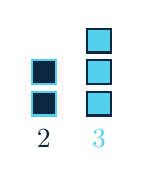
\begin{tikzpicture}
     \node[Tiber] at (0,-0.3) {$2$};
     \draw[draw=PictonBlue,thick,fill=Tiber] (-0.15,0) rectangle ++(.3,.3);
     \draw[draw=PictonBlue,thick,fill=Tiber] (-0.15,0.4) rectangle ++(.3,.3);

     \node[PictonBlue] at (0.7,-0.3) {$3$};
     \draw[draw=Tiber,thick,fill=PictonBlue] (0.55,0) rectangle ++(.3,.3);
     \draw[draw=Tiber,thick,fill=PictonBlue] (0.55,0.4) rectangle ++(.3,.3);
     \draw[draw=Tiber,thick,fill=PictonBlue] (0.55,0.8) rectangle ++(.3,.3);
    \end{tikzpicture}
   \end{subfigure}
   \pause
   \begin{subfigure}[b]{.2\textwidth}
    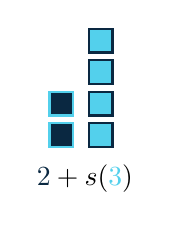
\begin{tikzpicture}
     \draw[draw=PictonBlue,thick,fill=Tiber] (-0.15,0) rectangle ++(.3,.3);
     \draw[draw=PictonBlue,thick,fill=Tiber] (-0.15,0.4) rectangle ++(.3,.3);

     \node at (0.3,-0.4) {$\clt{2} + s(\clp{3})$};
     \draw[draw=Tiber,thick,fill=PictonBlue] (0.35,0) rectangle ++(.3,.3);
     \draw[draw=Tiber,thick,fill=PictonBlue] (0.35,0.4) rectangle ++(.3,.3);
     \draw[draw=Tiber,thick,fill=PictonBlue] (0.35,0.8) rectangle ++(.3,.3);
     \draw[draw=Tiber,thick,fill=PictonBlue] (0.35,1.2) rectangle ++(.3,.3);
    \end{tikzpicture}
   \end{subfigure}
   \pause
   \begin{subfigure}[b]{.2\textwidth}
    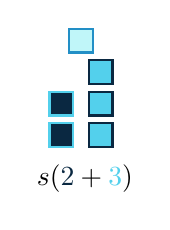
\begin{tikzpicture}
     \draw[draw=PictonBlue,thick,fill=Tiber] (-0.15,0) rectangle ++(.3,.3);
     \draw[draw=PictonBlue,thick,fill=Tiber] (-0.15,0.4) rectangle ++(.3,.3);

     \node at (0.3,-0.4) {$s(\clt{2} + \clp{3})$};
     \draw[draw=Tiber,thick,fill=PictonBlue] (0.35,0) rectangle ++(.3,.3);
     \draw[draw=Tiber,thick,fill=PictonBlue] (0.35,0.4) rectangle ++(.3,.3);
     \draw[draw=Tiber,thick,fill=PictonBlue] (0.35,0.8) rectangle ++(.3,.3);

     \draw[draw=CuriousBlue,thick,fill=Charlotte] (0.1,1.2) rectangle ++(.3,.3);
    \end{tikzpicture}
   \end{subfigure}
  \end{figure}
  \pause
  Using the formula $n + s(m) = s(n + m)$, one calculates $a + b$ by taking the
  successor of $a$ $b$ times.
  \pause
  Like this:
  \begin{align*}
   a + 0 &= a,\\
   a + 1 &= a + s(0) = s(a + 0) = s(a),\\
   a + 2 &= a + s(1) = s(a + 1) = s(a + s(0)) = s(s(a + 0)) = s(s(a)),\\
   \vdots&
  \end{align*}
\end{frame}

\begin{frame}
 \frametitle{Addition -- Properties}
 Addition of natural numbers satisfies these two properties:
 \begin{itemize}[label=\textbullet]
  \item \alert{Commutativity}:
  \[
   a + b = b + a.
  \]
 \pause
 \item \alert{Associativity}:
 \[
  a + (b + c) = (a + b) + c.
 \]
 \end{itemize}
\end{frame}

\begin{frame}
 \frametitle{Addition -- Properties}
 Using blocks, \alert{commutativity} just means that putting $a$ blocks next to
 $b$ blocks is the same as putting $b$ blocks next to $a$ blocks.
 \pause
 \begin{figure}[ht]
  \centering
  \begin{subfigure}[b]{.2\textwidth}
   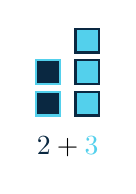
\begin{tikzpicture}
    \draw[draw=PictonBlue,thick,fill=Tiber] (-0.15,0) rectangle ++(.3,.3);
    \draw[draw=PictonBlue,thick,fill=Tiber] (-0.15,0.4) rectangle ++(.3,.3);

    \node at (0.25,-0.4) {$\clt{2} + \clp{3}$};
    \draw[draw=Tiber,thick,fill=PictonBlue] (0.35,0) rectangle ++(.3,.3);
    \draw[draw=Tiber,thick,fill=PictonBlue] (0.35,0.4) rectangle ++(.3,.3);
    \draw[draw=Tiber,thick,fill=PictonBlue] (0.35,0.8) rectangle ++(.3,.3);
   \end{tikzpicture}
  \end{subfigure}
  \pause
  \begin{subfigure}[b]{.2\textwidth}
   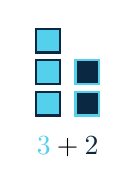
\begin{tikzpicture}
    \node at (0.25,-0.4) {$\clp{3} + \clt{2}$};
    \draw[draw=Tiber,thick,fill=PictonBlue] (-0.15,0) rectangle ++(.3,.3);
    \draw[draw=Tiber,thick,fill=PictonBlue] (-0.15,0.4) rectangle ++(.3,.3);
    \draw[draw=Tiber,thick,fill=PictonBlue] (-0.15,0.8) rectangle ++(.3,.3);

    \draw[draw=PictonBlue,thick,fill=Tiber] (0.35,0) rectangle ++(.3,.3);
    \draw[draw=PictonBlue,thick,fill=Tiber] (0.35,0.4) rectangle ++(.3,.3);
   \end{tikzpicture}
  \end{subfigure}
 \end{figure}
\end{frame}

\begin{frame}
 \frametitle{Addition -- Properties}
 Using blocks, \alert{associativity} just means that putting $b$ blocks next to
 $c$ blocks and then $a$ more blocks next to those is the same as putting $b$
 blocks next to $a$ blocks and then $c$ more blocks next to those.
 \begin{figure}[ht]
  \centering
  \begin{subfigure}[b]{.2\textwidth}
   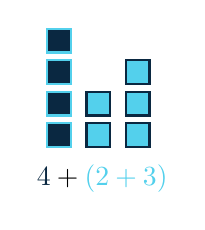
\begin{tikzpicture}
    \draw[draw=PictonBlue,thick,fill=Tiber] (-0.15,0) rectangle ++(.3,.3);
    \draw[draw=PictonBlue,thick,fill=Tiber] (-0.15,0.4) rectangle ++(.3,.3);
    \draw[draw=PictonBlue,thick,fill=Tiber] (-0.15,0.8) rectangle ++(.3,.3);
    \draw[draw=PictonBlue,thick,fill=Tiber] (-0.15,1.2) rectangle ++(.3,.3);

    \node at (0.55,-0.4) {$\clt{4} + \clp{(2 + 3)}$};
    \draw[draw=Tiber,thick,fill=PictonBlue] (0.35,0) rectangle ++(.3,.3);
    \draw[draw=Tiber,thick,fill=PictonBlue] (0.35,0.4) rectangle ++(.3,.3);

    \draw[draw=Tiber,thick,fill=PictonBlue] (0.85,0) rectangle ++(.3,.3);
    \draw[draw=Tiber,thick,fill=PictonBlue] (0.85,0.4) rectangle ++(.3,.3);
    \draw[draw=Tiber,thick,fill=PictonBlue] (0.85,0.8) rectangle ++(.3,.3);
   \end{tikzpicture}
  \end{subfigure}
  \pause
  \begin{subfigure}[b]{.2\textwidth}
   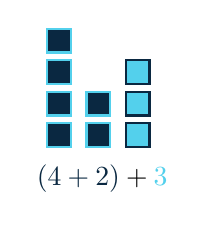
\begin{tikzpicture}
    \draw[draw=PictonBlue,thick,fill=Tiber] (-0.15,0) rectangle ++(.3,.3);
    \draw[draw=PictonBlue,thick,fill=Tiber] (-0.15,0.4) rectangle ++(.3,.3);
    \draw[draw=PictonBlue,thick,fill=Tiber] (-0.15,0.8) rectangle ++(.3,.3);
    \draw[draw=PictonBlue,thick,fill=Tiber] (-0.15,1.2) rectangle ++(.3,.3);

    \node at (0.55,-0.4) {$\clt{(4 + 2)} + \clp{3}$};
    \draw[draw=PictonBlue,thick,fill=Tiber] (0.35,0) rectangle ++(.3,.3);
    \draw[draw=PictonBlue,thick,fill=Tiber] (0.35,0.4) rectangle ++(.3,.3);

    \draw[draw=Tiber,thick,fill=PictonBlue] (0.85,0) rectangle ++(.3,.3);
    \draw[draw=Tiber,thick,fill=PictonBlue] (0.85,0.4) rectangle ++(.3,.3);
    \draw[draw=Tiber,thick,fill=PictonBlue] (0.85,0.8) rectangle ++(.3,.3);
   \end{tikzpicture}
  \end{subfigure}
 \end{figure}
\end{frame}

\end{document}
